\UseRawInputEncoding
\documentclass[lettersize,journal]{IEEEtran}
%\documentclass[lettersize,journal,onecolumn]{IEEEtran}
\usepackage{amsmath,amsfonts}
\usepackage{algorithmic}
\usepackage{algorithm}
\usepackage{amsmath}
\usepackage{array}
\usepackage[caption=false,font=normalsize,labelfont=sf,textfont=sf]{subfig}
\usepackage{textcomp}
\usepackage{stfloats}
\usepackage{url}
\usepackage{verbatim}
\usepackage{graphicx}
\usepackage{cite}
\usepackage{epsfig}
\usepackage{bm}
\usepackage{makecell}
%\linespread{2}
\usepackage{multirow}
\hyphenation{op-tical net-works semi-conduc-tor IEEE-Xplore}
% updated with editorial comments 8/9/2021

\begin{document}

\title{Low-complexity Resource Allocation for User Paired RSMA in Future 6G Wireless Networks}

\author{\thanks{This work is jointly supported by NSFC project (grant No.61971359), Chongqing Municipal Key Laboratory of Institutions of Higher Education (grant No. cqupt-mct-202104).}
Jiewen Hu\thanks{Jiewen Hu is currently pursuing the Ph.D. degree at School of Information Science and Technology, Southwest Jiaotong University, China. (email: jevon@my.swjtu.edu.cn).},
Gang Liu\thanks{Gang Liu is currently an associate professor at School of Information Science and Technology, Southwest Jiaotong University, China. (email: gangliu@swjtu.edu.cn).}, \emph{Member, IEEE},
Zheng Ma\thanks{Zheng Ma is currently a professor at School of Information Science and Technology, Southwest Jiaotong University, China. (zma@home.swjtu.edu.cn).}, \emph{Member, IEEE},
Ming Xiao\thanks{Ming Xiao is with the Department of Information, Science and Engineering,
School of Electrical Engineering, KTH, 10044 Stockholm, Sweden (e-mail:
mingx@kth.se).}, \emph{Senior Member, IEEE},
and Pingzhi Fan\thanks{Pingzhi Fan is currently a distinguished professor at Southwest Jiaotong University, China. (pzfan@swjtu.edu.cn).}, \emph{Fellow, IEEE}
}
%,  Yongbo Li, Zheng Ma, Wei Wang, Chengchao Liang, F. Richard Yu and Pingzhi Fan}
 %}        %<-this % stops a space
%\thanks{This paper was produced by the IEEE Publication Technology Group. They are in Piscataway, NJ.}% <-this % stops a space
%\thanks{.}}
%\thanks{Jiewen Hu is currently pursuing the Ph.D. degree at School of Information Science and Technology, Southwest Jiaotong University, China.}



%Gang Liu [M'15] is currently an associate professor at School of Information Science and Technology, Southwest Jiaotong University, China.}


% The paper headers
%\markboth{Journal of \LaTeX\ Class Files,~Vol.~14, No.~8, August~2021}%
%{Shell \MakeLowercase{\textit{et al.}}: A Sample Article Using IEEEtran.cls for IEEE Journals}

%\IEEEpubid{0000--0000/00\$00.00~\copyright~2021 IEEE}
% Remember, if you use this you must call \IEEEpubidadjcol in the second
% column for its text to clear the IEEEpubid mark.

\maketitle

\begin{abstract}

%Railway communication is an essential way to ensure the safety of railway transportation. The Global System for Mobile Communications - Railway (GSM-R) is widely used for railway communication. However, GSM-R is predicted to be obsoleted by 2030, and a suitable successor is needed. Defined by the International Union of Railways (UIC), the Future Railway Mobile Communication System (FRMCS) contains many future use cases with strict requirements. These use cases should ensure regular communication not only in network coverage but also uncovered scenarios. There is still a lack of standards on off-network communication in FRMCS, so this article focuses on off-network communication and intends to provide reference and direction for standardization. We first provide a comprehensive summary and analysis of off-network use cases in FRMCS. Then we give an overview of existing technologies (GSM-R, TETRA, DMR, LTE-V2X, and NR-V2X) that may support off-network communication and discuss their physical layer characteristics. In addition, we simulate and evaluate the performance of existing technologies. Simulation results show that it is possible to satisfy the off-network communication requirements in FRMCS with enhancements based on LTE-V2X or NR-V2X. Finally, we give some future research directions to provide insights for industry and academia.
Rate-splitting multiple access (RSMA) uplink requires optimization of decoding order and power allocation, while decoding order is a discrete variable, and it is very complex to find the optimal decoding order if the number of users is large enough. This letter proposes a low-complexity user pairing-based resource allocation algorithm with the objective of minimizing the maximum latency, which significantly reduces the computational complexity and also achieves similar performance to unpaired uplink RSMA. A closed-form expression for power and bandwidth allocation is first derived, and then a bisection method is used to determine the optimal resource allocation. Finally, the proposed algorithm is compared with unpaired RSMA, paired NOMA and unpaired NOMA. The results demonstrate the effectiveness of the proposed algorithm.
\end{abstract}

\begin{IEEEkeywords}
rate-splitting multiple access (RSMA), decoding order, user pairing, resource allocation, 6G Wireless Networks.
\end{IEEEkeywords}
\section{Introduction}
6G takes the upper bound of wireless access capacity to a new level, and it expects ubiquitous connectivity, which is overwhelming for existing systems. An excellent multiple access schemes can effectively solve the above problems, and RSMA is a promising multiple access scheme recently.

RSMA splits the message at the transmitter and transmits it by superposition coding, then decodes it at the receiver using successive interference cancellation (SIC). In RSMA downlink, the message of each user is split into a private part and a common part, and the common part of all users is encoded into one common stream and transmitted superimposed with the private stream of each user at the transmitter side. After users receive the message, the common stream is first decoded by treating all users' private streams as noise, then the interference of common streams to private streams is removed by using SIC, and finally the private stream is decoded by treating other users' private streams as noise\cite{ref1}. The RSMA downlink is heavily researched, but the uplink has not been well investigated, so this letter focuses on the RSMA uplink.

In the RSMA uplink, the message of each user is split into two parts, each part is encoded independently and transmitted superimposed. The SIC technique is used at the base station for decoding in a specified decoding order \cite{ref2}. In existing works on RSMA uplink, the authors in \cite{ref3} studied the performance of two-user uplink RSMA in terms of outage probability and achievable sum rate, and gave the exact closed-form expression. In \cite{ref4}, fixed rate splitting (FRS) and cognitive rate splitting (CRS) for two-user uplink are studied to improve user fairness and outage performance, and a closed-form expression for the outage probability is given. The authors in \cite{ref5} investigated reconfigurable intelligent surface (RIS)-assisted two-user RSMA uplink, and optimized the transmit power and beamforming with the objective of maximizing the achievable rate. \cite{ref6} studied the two-user RSMA uplink, which first derives closed-form expressions for outage probabilities and then uses them to derive user throughput with a medium access control protocol based on the slotted ALOHA and RSMA. Cooperative NOMA (C-NOMA) and cooperative RSMA (C-RSMA) for two user uplink were proposed in \cite{ref7} and the proportional fairness coefficient was considered to formulate two optimization problems for comparison.

All above studies are based on two users. However, when the number of users is large enough, the optimal decoding order of RSMA uplink is a mixed integer nonlinear programming, and there is lack of effective way to solve it. The authors in \cite{ref8} optimized the power allocation and passive beamforming for users of RIS-assisted uplink RSMA systems with the objective of maximization sum-rate, and proposed a suboptimal decoding order based on channel gain and message splitting ratio. \cite{ref9} adopted an exhaustive search method to find the optimal decoding order and introduced user pairing to reduce the complexity of the algorithm.

Most of the existing researches focus on user fairness, sum rate or interruption probability, while in some automatic control scenarios, latency is a more important parameter, such as automatic control of vehicle platooning, where the lead vehicle needs to wait to collect the movement status of all platooning vehicles before making control decisions, which needs to minimize the maximum latency for all users. In addition, the complexity of existing algorithms should be further reduced.

In this letter, we optimize the uplink RSMA with the objective of minimizing the maximum latency. Since the optimal decoding order is difficult to find, user pairing is employed to reduce the computational complexity. Then the optimization variables are changed from decoding order and power allocation to bandwidth allocation and power allocation, by making use of the fact that the optimal decoding order of two users can be determined. We derive the closed-form expressions for power and bandwidth allocation, respectively, and the optimal solution of the optimization problem is obtained by bisection method. Finally, the effectiveness of the algorithm is verified by simulation.
\section{SYSTEM MODEL AND PROBLEM FORMULATION}
%\subsection{RSMA uplink without user pairing}
Without loss of generality, this letter considers a single input single output (SISO) uplink RSMA transmission as shown in Fig. \ref{fig:1}, which contains a base station (BS) and $N$ users. The channel gain from the user $n$ to BS is denoted by $h_{n}$. Using RSMA uplink transmission, the information $x_n$ of user $n$ is divided into $x_{n1}$ and $x_{n2}$. The message received by BS can be expressed as $y_{BS}=\sum^{N}_{n=1}\sum^{2}_{j=1}{\sqrt{h_{n}}\cdot x_{nj}}+n_{0}$, where $n_{0}$ denotes additive Gaussian white noise. After SIC is performed at BS, the rate of $x_{nj}$ can be expressed as $r_{nj}=B\log_{2}(1+\frac{h_np_{nj}}{\sum_{\{(n'\in N,j'\in J)\mid\pi_{n'j'}>\pi_{nj}\}}h_{n'}p_{n'j'}+\sigma^{2}B})$, where $B$ is the bandwidth, $p_{nj}$ is the transmission power allocated to $x_{nj}$, $\pi_{nj}$ is the decoding order of $x_{nj}$, and $\sigma^{2}$ is the power spectral density of the Gaussian noise. So the transmission rate of user $n$ can be expressed as $r_{n}=\sum^2_{j=1}r_{nj}$, and the transmission latency can be write as $t_n={PL}_n/r_n$, where ${PL}_n$ is the package length of user $n$.
%\iffalse \fi%��ע��
\begin{figure}[!t]
\centering
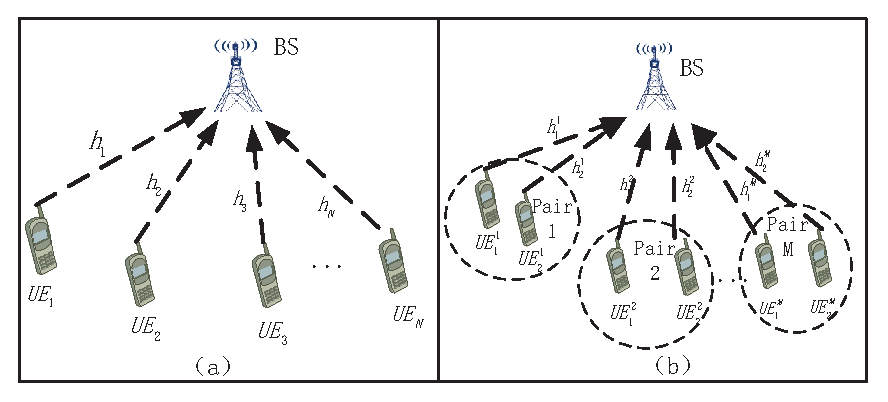
\includegraphics[width=3.5in]{fig1}
\caption{(a) Uplink RSMA without user pairing. (b) Uplink RSMA with user pairing.}
\label{fig:1}
\end{figure}
In some automatic control systems, the BS needs to obtain information from all users before making control decisions, so we build the following optimization problem to minimize the maximum transmission latency.
\begin{align}\label{eq1}
\boldsymbol{P1}: \hspace{10mm}  &\min_{\boldsymbol{\pi}\boldsymbol{p}}\max\quad t_n \\
s.t.  \ \ &\  p_{nj}>0, 1\leq n \leq N, j\in[1,2];\tag{1a}\\
            &\ \boldsymbol{\pi} \in\mathbf{\Pi};  \tag{1b}\\%\notag,
            &\  \sum^{2}_{j=1} p_{nj}\leq P^{max}_n, 1\leq n \leq N. \tag{1c}
\end{align}
where $\boldsymbol{p}=[p_{11},p_{12},p_{21},...,p_{n2}]$, $\mathbf{\Pi}$ denotes all possible orders of decoding and $P^{max}_n$ is the maximum transmission power of user n.

Using $\tau$ to denote the upper bound of latency for all users, we have $t_n\leq \tau, 1\leq n \leq N$, Then problem $\boldsymbol{P1}$ can be transformed into:
\begin{align}\label{eq2}
\boldsymbol{P2}: \hspace{10mm}  &\min_{\boldsymbol{\pi}\boldsymbol{p}} \tau \\
s.t.  \ \ &\  r_{n}\geq\frac{{PL}_n}{\tau}, 1\leq n \leq N, j\in[1,2];\tag{2a}\\
           %  &\ (1a),(1b),(1c).
            &\  p_{nj}>0, 1\leq n \leq N, j\in[1,2];\tag{2b}\\
            &\ \boldsymbol{\pi}\in\Pi;  \tag{2c}\\%\notag,
            &\  \sum^{2}_{j=1} p_{nj}\leq P^{max}_n, 1\leq n \leq N; \tag{2d}
\end{align}
The decoding order $\boldsymbol{\pi}$ in problem $\boldsymbol{P2}$ is a discrete variable, and the condition (2a) is in the form of the sum of two logarithmic functions. We can exhaust $\boldsymbol{\pi}$ and use the successive convex approximation (SCA) algorithm to transform condition (2a) into a convex form to find the approximate solution. However, the decoding order set $\boldsymbol{\Pi}$ contains $(2N)!/2^{N}$ elements, which means that the complexity of the algorithm using the exhaustive method will become extremely high as the number of users increases. Existing studies have determined the optimal decoding order of RSMA transmissions for two users\cite{ref9}, so we consider pairing every two users to reduce the complexity of the algorithm.

%\subsection{User pairing and power allocation in RSMA}
As show in part (b) of Fig. \ref{fig:1}, suppose all users are paired into $M$ pairs, and each pair contains two users. According to the simulation test, since the change of channel gain is much larger than package length, the performance of pairing mainly depends on the channel gains, so this pairing is performed according to the order of channel gains\cite{ref10}. The channel gain of the $k$-th user in the $m$-th pair to the BS is denoted by $h_{k}^{m},k\in[1,2], 1\leq m \leq M$. Research \cite{ref11} shows that uplink RSMA transmission of two users can achieve all rate regions by splitting the information of only one user. Without loss of generality, suppose the message of the first user in each pair is split into two parts $x^m_{11}$ and $x^m_{12}$ , and the message of the second user is not split, the optimal decoding order at the BS is $x^m_{11}$, $x^m_{2}$, $x^m_{12}$.

The following is an analysis for the m-th pair of users. the rate of $x^m_{11}$, $x^m_{2}$ and $x^m_{12}$ can be expressed respectively as:
\begin{equation}\label{eq3}
r^m_{11}=B\alpha_m \log_2(1+\frac{h^m_1 p^m_{11}}{h^m_2p^m_2+h^m_1p^m_{12}+\sigma^2B\alpha_m}),\\
\end{equation}
\begin{equation}\label{eq4}
r^m_{2}=B\alpha_m \log_2(1+\frac{h^m_2p^m_2}{h^m_1p^m_{12}+\sigma^2B\alpha_m}),\\
\end{equation}
\begin{equation}\label{eq5}
r^m_{12}=B\alpha_m \log_2(1+\frac{h^m_1p^m_{12}}{\sigma^2B\alpha_m}),\\
\end{equation}
where $\alpha_m$ is the bandwidth allocation factor with $\sum_{m=1}^{M}\alpha_m\leq1$, $p^m_{11}$, $p^m_{2}$ and $p^m_{12}$ are the power allocated to $x^m_{11}$, $x^m_{2}$ and $x^m_{12}$ respectively. So the rate of user 1 in m-th pair is $r^m_1=r^m_{11}+r^m_{12}$ and the transmission latency of user $k$ in the $m$-th pair is $t^m_k=PL^m_k/r^m_K$, where ${PL}^m_k$ is the package length of user $k$ in the $m$-th pair.

The optimization of the power and decoding order in $\boldsymbol{P2}$  can be translated into the optimization of the bandwidth and power allocation in $\boldsymbol{P3}$  as follows:
\begin{align}\label{eq6}
\boldsymbol{P3}: \hspace{10mm}  &\min_{\boldsymbol{\alpha}\boldsymbol{p}}\quad \tau \\
s.t.  \ \   &\ r^m_{k}\geq\frac{PL^m_k}{\tau}, 1\leq m \leq M, k\in[1,2];\tag{6a}\\
            &\  p^m_{kj}>0, 1\leq m \leq M, k,j\in [1,2];\tag{6b}\\
            &\ \sum^M_{m=1} \alpha_m \leq 1;  \tag{6c}\\%\notag,
            &\  \sum^{2}_{j=1} p^m_{kj}\leq P^m_{kmax}, 1\leq m \leq M, k,j\in[1,2]; \tag{6d}
\end{align}
\section{RESOURCE ALLOCATION ALGORITHM FOR PAIRED RSMA}
Since the expression of transmission rate is a monotonically increasing function of power and bandwidth, we can use contradiction to prove that the optimal solution of $\boldsymbol{P3}$ is obtained when and only when all users have the same latency, i.e., $t^1_1:t^1_2:t^2_1:...:t^M_2=1:1:1:...:1$, in other words, the ratio of optimized rates is $r^1_1:r^1_2:r^2_1:...:r^M_2={PL}^1_1:{PL}^1_2:{PL}^2_1:...:{PL}^M_2$. Thus, the rates of two users in the same pair have $r^m_2=\frac{{PL}^m_2}{{PL}^m_1}r^m_1$.

\begin{figure}[!t]
\centering
\includegraphics[width=2.5in]{fig2}
\caption{Rate region of $r_1$ and $r_2$ in the same pair when use RSMA}
\label{fig:2}
\end{figure}

Fig. \ref{fig:2} shows the achievable rate region for two users using RSMA transmission, when the decoding order is $x^m_{11}$, $x^m_{2}$ and $x^m_{12}$, all points on the rate region can be reached:

For the line AB, the power allocation is:
\begin{equation}\label{eq7}
0\leq p^m_{11}\leq P^m_{1max},\quad p^m_{12}=0,\quad p^m_{2}=P^m_{2max},\\
\end{equation}
User 2 has the maximum rate as:
\begin{equation}\label{eq8}
 r^m_{2}=B\alpha_m \log_2(1+\frac{h^m_2P^m_{2max}}{\sigma^2B\alpha_m}).
\end{equation}

For the line BC, the power allocation is:
\begin{equation}\label{eq9}
p^m_{11}+ p^m_{12}=P^m_{1max},\quad p^m_{2}=P^m_{2max},\\
\end{equation}
The sum rate of the two user is:
\begin{equation}\label{eq10}
r^m_{1}+r^m_{2}=B\alpha_m \log_2(1+\frac{h^m_1P^m_{1max}+h^m_2P^m_{2max}}{\sigma^2B\alpha_m}).
\end{equation}

For the line CD, the power allocation is:
\begin{equation}\label{eq11}
p^m_{11}=0,\quad p^m_{12}=P^m_{1max},\quad 0\leq p^m_{2}\leq P^m_{2max},\\
\end{equation}
User 1 has the maximum rate as :
\begin{equation}\label{eq12}
r^m_{1}=B\alpha_m \log_2(1+\frac{h^m_1P^m_{1max}}{\sigma^2B\alpha_m}).
\end{equation}

According to the above analysis, the optimal power allocation of problem $\boldsymbol{P3}$ is the intersection of line $r^m_2=\frac{{PL}^m_2}{{PL}^m_1}r^m_1$ and the rate region. As shown in Fig. \ref{fig:2}, the intersection point may exist three cases.

\iffalse %��ע��
The intersection point is on AB when (13) is satisfied, on BC when (14) is satisfied, and on CD when (15) is satisfied
\begin{equation}\label{eq13}
r^m_{B2}<\frac{{PL}^m_2}{{PL}^m_1}r^m_{B1},\quad r^m_{C2}<\frac{{PL}^m_2}{{PL}^m_1}r^m_{C1}.
\end{equation}
\begin{equation}\label{eq14}
r^m_{B2}>\frac{{PL}^m_2}{{PL}^m_1}r^m_{B1},\quad r^m_{C2}<\frac{{PL}^m_2}{{PL}^m_1}r^m_{C1}.
\end{equation}
\begin{equation}\label{eq15}
r^m_{B2}>\frac{{PL}^m_2}{{PL}^m_1}r^m_{B1},\quad r^m_{C2}>\frac{{PL}^m_2}{{PL}^m_1}r^m_{C1}.
\end{equation}
where $r^m_{Bk}$,$r^m_{Ck}$ denote the rate of user k at points B and C respectively. According to (\ref{eq7}), (\ref{eq9}) and (\ref{eq11}), it can be derived that:
\begin{equation}\label{eq16}
\left\{
\begin{aligned}
r^m_{B1}=B\alpha_m \log_2(1+\frac{h^m_1P^m_{1max}}{h^m_2P^m_{2max}+\sigma^2B\alpha_m}).\\
r^m_{B2}=B\alpha_m \log_2(1+\frac{h^m_2P^m_{2max}}{\sigma^2B\alpha_m}).\\
\end{aligned}
\right.
\end{equation}

\begin{equation}\label{eq17}
\left\{
\begin{aligned}
r^m_{C1}=B\alpha_m \log_2(1+\frac{h^m_1P^m_{1max}}{\sigma^2B\alpha_m}).\\
r^m_{C2}=B\alpha_m \log_2(1+\frac{h^m_2P^m_{2max}}{h^m_1P^m_{1max}+\sigma^2B\alpha_m}).\\
\end{aligned}
\right.
\end{equation}
\fi


Case 1: The intersection point is on AB, and according to (\ref{eq3}), (\ref{eq7}), (\ref{eq8}) and (6a), we have:
\begin{equation}\label{eq13}
B\alpha^{AB}_m \log_2(1+\frac{h^m_2P^m_{2max}}{\sigma^2B\alpha^{AB}_m})=\frac{{PL}^m_2}{\tau},
\end{equation}
\begin{equation}\label{eq14}
p^m_{11}=\frac{(2^\frac{{PL}^m_1}{\tau B\alpha^{AB}_m}-1)(h^m_2P^m_2max+\sigma^2B\alpha^{AB}_m)}{h^m_1}.
\end{equation}


Case 2: The intersection point is on BC, and according to (\ref{eq4}), (\ref{eq9}), (\ref{eq10}) and (6a):
\begin{equation}\label{eq15}
B\alpha^{BC}_m \log_2(1+\frac{h^m_1P^m_{1max}+h^m_2P^m_{2max}}{\sigma^2B\alpha^{BC}_m})=\frac{{PL}^m_1+{PL}^m_2}{\tau},
\end{equation}

\begin{equation}\label{eq16}
p^m_{12}=\frac{h^m_2P^m_{2max}}{h^m_1(2^\frac{{PL}^m_2}{\tau B\alpha^{BC}_m}-1)}-\frac{\sigma^2B\alpha^{BC}_m}{h^m_1},
\end{equation}
The $r^m_{12}$ can be obtained by taking $p^m_{12}$ into (\ref{eq5}), then $r^m_{11}={PL}^m_1/ \tau- r^m_{12}$, and according to (\ref{eq3}) we can obtain $p^m_{11}$:
\begin{equation}\label{eq17}
p^m_{11}=\frac{(2^\frac{r^m_{11}}{B\alpha^{BC}_m}-1)(h^m_2P^m_{2max}+h^m_1p^m_{12}+\sigma^2B\alpha^{BC}_m)}{h^m_1}.
\end{equation}

Case 3: The intersection point is on CD, and according to (\ref{eq11}), (\ref{eq12}) and (6a):
\begin{equation}\label{eq18}
B\alpha^{CD}_m \log_2(1+\frac{h^m_1P^m_{1max}}{\sigma^2B\alpha^{CD}_m})=\frac{{PL}^m_1}{\tau},
\end{equation}
\begin{equation}\label{eq19}
p^m_{2}=\frac{(2^\frac{{PL}^m_2}{\tau B\alpha^{CD}_m}-1)(h^m_1P^m_1max+\sigma^2B\alpha^{CD}_m)}{h^m_2}.
\end{equation}

According to (\ref{eq13}), (\ref{eq15}) and (\ref{eq18}), the expression of $\alpha^{AB}_m$,$\alpha^{BC}_m$ and $\alpha^{CD}_m$ are given in (\ref{eq20}), (\ref{eq21}) and (\ref{eq22}).
\begin{figure*}[ht] %hb�����������µײ���%htΪ�������¶���
	\begin{equation}\label{eq20}
	\alpha^{AB}_m = \frac{-\ln2h^m_2P^m_{2max}{PL}^m_2}{\tau Bh^m_2P^m_{2max}W(\frac{-\ln2{PL}^m_2\sigma^2}{\tau h^m_2P^m_{2max}}e^{\frac{-\ln2{PL}^m_2\sigma^2}{\tau h^m_2P^m_{2max}}})+\ln2{PL}^m_2\sigma^2B},
	\end{equation}
	\begin{equation}\label{eq21}
\alpha^{BC}_m = \frac{-\ln2(h^m_1P^m_{1max}+h^m_2P^m_{2max})({PL}^m_1+{PL}^m_2)}{\tau B(h^m_1P^m_{1max}+h^m_2P^m_{2max})W(\frac{-\ln2({PL}^m_1+{PL}^m_2)\sigma^2}{\tau (h^m_1P^m_{1max}+h^m_2P^m_{2max})}e^{\frac{-\ln2({PL}^m_1+{PL}^m_2)\sigma^2}{\tau (h^m_1P^m_{1max}+h^m_2P^m_{2max})}})+\ln2({PL}^m_1+{PL}^m_2)\sigma^2B},
	\end{equation}
	\begin{equation}\label{eq22}
	\alpha^{CD}_m = \frac{-\ln2h^m_1P^m_{1max}{PL}^m_1}{\tau Bh^m_1P^m_{1max}W(\frac{-\ln2{PL}^m_1\sigma^2}{\tau h^m_1P^m_{1max}}e^{\frac{-\ln2{PL}^m_1\sigma^2}{\tau h^m_1P^m_{1max}}})+\ln2{PL}^m_1\sigma^2B},
	\end{equation}
\end{figure*}
Where $W(\cdot)$ is the Lambert-W function which satisfies $W(xe^x)=x$. Note that the Lambert-W function has multiple solutions here, and the appropriate solution should be chosen.

With the closed-form expressions for bandwidth allocation and power allocation, we can solve the problem $\boldsymbol{P3}$ by the bisection method. For each given $\tau$, a set of $\alpha^{AB}_m$, $\alpha^{BC}_m$ and $\alpha^{CD}_m$ can be calculated according to (\ref{eq20}), (\ref{eq21}) and (\ref{eq22}), and the power allocation corresponding to each case can be obtained by (\ref{eq14}), (\ref{eq16}), (\ref{eq17}) and (\ref{eq19}), and then the condition (6d) is used to judge which case occurs. The specific algorithm is shown in Algorithm 1.
\begin{algorithm}
   \caption{User pairing-based power allocation algorithm.}
   \begin{algorithmic}[1]
   \STATE {Initialize upper and lower bound $\tau_{ub}$, $\tau_{lb}$, tolerance $\varepsilon$.}
   \WHILE{ $\tau_{ub}-\tau_{lb}>\varepsilon$ }
       \STATE set   $ \tau=\frac{\tau_{ub}+\tau_{lb}}{2}$
       \FOR{m=1:$M$}
       \STATE calculate $\alpha^{AB}_m$, $\alpha^{BC}_m$ and $\alpha^{CD}_m$ respectively according to (\ref{eq20}), (\ref{eq21}) and (\ref{eq22}).
       \STATE Calculate the power allocation for each case according to (\ref{eq14}), (\ref{eq16}), (\ref{eq17}) and (\ref{eq19}) respectively.

       \IF {The power allocation of case 1 satisfies (6d)}
           \STATE $\alpha_m=\alpha^{AB}_m$.

       \ELSIF {The power allocation of case 2 satisfies (6d)}
            \STATE $\alpha_m=\alpha^{BC}_m$.
       \ELSIF {The power allocation of case 3 satisfies (6d)}
            \STATE $\alpha_m=\alpha^{CD}_m$.
            \ELSE
            \STATE set $\tau_{lb}=\tau$, break and jump to step 2.
       \ENDIF
       \ENDFOR
        \IF {$\sum_{m=1}^{M}\alpha_m\leq1$}
        \STATE set $\tau_{ub}=\tau$.
        \ELSE
        \STATE set $\tau_{lb}=\tau$.
        \ENDIF
   \ENDWHILE
   \STATE {Output $\tau$, $\alpha_m$, $p^m_{11}$, $p^m_{12}$, and $p^m_{2}$.}
   \end{algorithmic}
   \end{algorithm}

The complexity of Algorithm 1 in each iteration is to check which case satisfies the power constraint (6d), which introduces the complexity of $ \mathcal{O}(M)$ according to (\ref{eq14}), (\ref{eq16}), (\ref{eq17}) and (\ref{eq19})-(\ref{eq22}). In addition the complexity of the bisection method with accuracy $\varepsilon$ is $ \mathcal{O}(\log_2(1/\varepsilon))$\cite{ref12}, so the total complexity of Algorithm 1 is $ \mathcal{O}(M\log_2(1/\varepsilon))$.

\section{SIMULATION RESULT AND DISCUSSIONS}
We simulate the proposed algorithm in this section. $N$ users are uniformly distributed within a radius of 200 m from the BS, and the path loss model is $128.1+37.6\log_{10}d$ ($d$ is in km). The bandwidth is set to 1 MHz, and the noise power spectral density is $\sigma^2=-174 $ dBm/Hz\cite{ref9}. Each user has the same power limit $P_{max}$ and randomly generates a packet of 50-1200 bytes. The algorithms for the comparison include unpaired RSMA\cite{ref8}, paired NOMA\cite{ref10} and unpaired NOMA. All simulation results were performed on an Intel Core i9-13900KF CPU @ 5.8 GHz and 32G RAM using MATLAB R2023a.
\begin{figure}[!t]
\centering
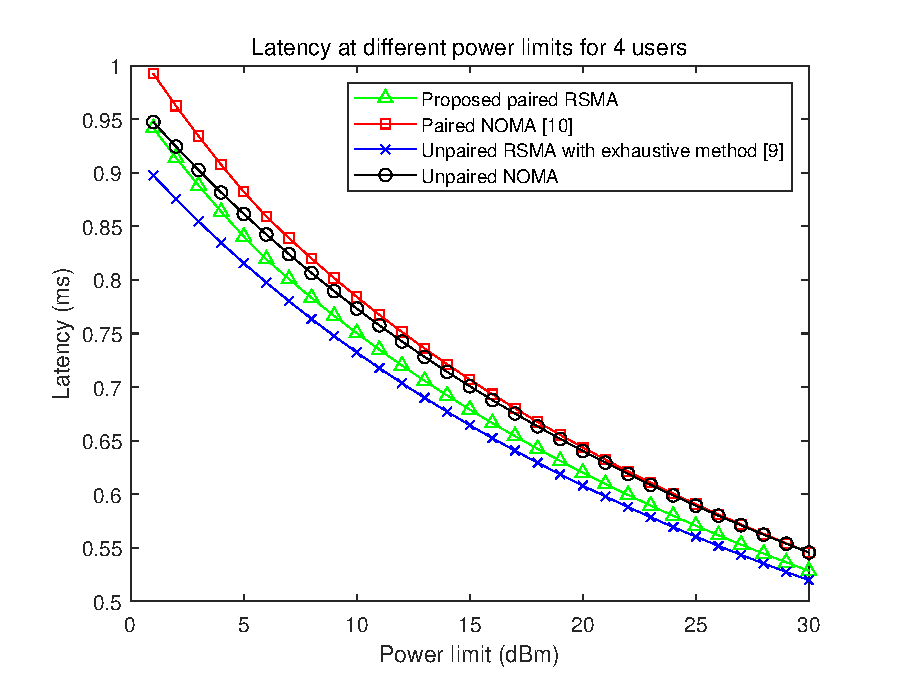
\includegraphics[width=3.5in]{fig3}
\caption{Latency performance with different power limits when the number of users $N=4$.}
\label{fig:3}
\end{figure}

Fig. \ref{fig:3} shows the transmission latency of each scheme with different power limits for the number of users $N=4$, where unpaired RSMA exhausts all decoding orders to obtain the optimal solution. As $P_{max}$ increases, the latency decreases for all schemes. It can be seen that RSMA outperforms NOMA, regardless of pairing or non-pairing, the reason is that NOMA is an extreme special case of RSMA, while RSMA can handle the resource allocation and decoding methods between different packets more flexibly to obtain better performance. In addition, the proposed paired RSMA resource allocation algorithm gives a closed-form solution for power and bandwidth allocation, which significantly reduces the computational complexity and has not much performance loss compared to the unpaired RSMA.

\begin{figure}[!t]
\centering
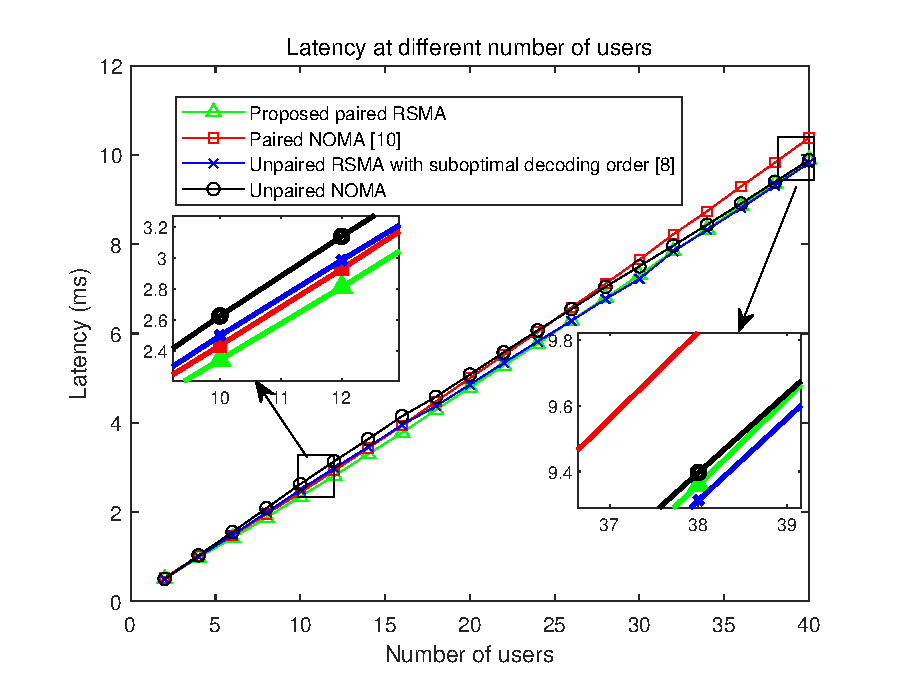
\includegraphics[width=3.5in]{fig4}
\caption{Latency performance for different total number of users when the power limit $P_{max}=23$ dBm.}
\label{fig:4}
\end{figure}

Since the algorithmic complexity of the exhaustive method grows exponentially as the total number of users increases, we choose a suboptimal decoding order \cite{ref8} to compare the latency performance at different total number of users in Fig. \ref{fig:4}, and the power limit is set to $P_{max}=23$ dBm. It can be seen that RSMA always outperforms NOMA, regardless of paired or unpaired. In addition, the paired schemes are more advantageous when the total number of users is small, and as the total number of users increases, the performance of the unpaired schemes will outperform the paired schemes due to the fact that more number of users means more number of pairs and therefore less bandwidth is allocated to each pair. Overall, the proposed paired-based RSMA resource allocation algorithm greatly reduces the complexity and achieves similar performance to unpaired RSMA.

%In addition,, and the performance gap increases with the growth of the total number of users. In addition, more number of users means more number of pairs and therefore less bandwidth is allocated to each pair, so the performance of the paired RSMA gets worse compared to the unpaired RSMA as the total number of users increases. Therefore the proposed algorithm is more suitable for the case where the total number of users is not particularly large. As shown in the figure, at 40 users, the proposed pairing-based RSMA resource allocation algorithm is only 0.5467 ms worse than the unpaired RSMA performance, which is within an acceptable range.
%& \makecell[c]{Paired NOMA} & \makecell[c]{Unpaired NOMA}& \makecell[c]{Unpaired RSMA with exhaustive method}\makecell[c]{ & Unpaired RSMA with suboptimal decoding order}
%\makecell[c]{Number of users \\(N)}
\begin{table}
\begin{center}
\caption{Comparison of the computational complexity of each scheme}
\label{tab1}
\setlength{\tabcolsep}{1mm}{
\begin{tabular}{| c | c | c | c | c | c |}
\hline
\multirow{2}*{Schemes} &\multicolumn{5}{c|}{Simulation time}\\
\cline{2-6}
~ & $N=4$ & $N=10$ & $N=20$& $N=30$ & $N=40$ \\
\hline
\makecell[c]{Proposed \\paired RSMA}& 0.068 s&0.095 s&0.106 s&0.141 s&0.131 s \\
\hline
\makecell[c]{Unpaired \\RSMA with \\exhaustive method}&3447.5 s & -& - & - & -\\
\hline
\makecell[c]{ Unpaired RSMA\\ with suboptimal \\decoding order}&1.783 s&7.378 s&19.002 s&36.117 s&74.457 s\\
\hline
\makecell[c]{Paired NOMA}&4.084 s&4.515 s&5.737 s&7.589 s&10.113 s\\
\hline
\makecell[c]{Unpaired NOMA}&4.031 s&4.260 s&4.603 s&5.106 s&5.271 s\\
\hline
\end{tabular}}
\end{center}
\end{table}


To further evaluate the benefits of the proposed algorithm in terms of complexity, Table \ref{tab1} gives the simulation time for each scheme at different total number of users. For unpaired RSMA, the algorithmic complexity introduced by the exhaustive decoding order method is unacceptable, and even given a suboptimal decoding order, the computational complexity grows rapidly when the number of users increases. On the contrary, the proposed paired RSMA algorithm gives a closed-form expression for power and bandwidth allocation, and achieves similar performance to unpaired RSMA with a very low complexity.

The results demonstrate that the proposed user pairing-based power allocation algorithm achieves good performance with significantly reduced computational complexity, As the total number of users increases, the performance of the proposed algorithm decreases due to the total bandwidth limitation, and the computational complexity of the unpaired uplink RSMA to confirm the optimal decoding order exponentially increases, so there is a trade-off between computational complexity and transmission performance.

\section{Conclusion}
In this letter, to address the requirement of maximum latency among all users in some automatic control scenarios, we propose a resource allocation algorithm for uplink RSMA to minimize the maximum transmission latency. However, the complexity of uplink RSMA to confirm the optimal decoding order grows exponentially with the total number of users, so user pairing is introduced and a low-complexity resource allocation algorithm based on user pairing is designed to transform the optimization of power and decoding order into the optimization of power and bandwidth allocation. The achievable rate region of two-user uplink RSMA is first analyzed, and the closed-form expressions of three possible values of the optimal power and bandwidth allocation are derived. Then the maximum latency $\tau$ is determined by the bisection method, and for each given $\tau$, the corresponding three power and bandwidth allocations are derived. The optimal power allocation scheme is determined by judging which one satisfies the power constraint. Results show that the proposed low-complexity algorithm based on user pairing significantly reduces the user complexity and also achieves similar performance to unpaired uplink RSMA.

%\section*{Acknowledgments}
%This work is jointly supported by NSFC project (grant No.61971359), Chongqing Municipal Key Laboratory of Institutions of Higher Education (grant No. cqupt-mct-202104), Fundamental Research Funds for the Central Universities, Sichuan Science and Technology Project (grant no. 2021YFQ0053) and State Key Laboratory of Rail Transit Engineering Informatization (FSDI).






%{\appendices
%\section*{Proof of the First Zonklar Equation}
%Appendix one text goes here.
% You can choose not to have a title for an appendix if you want by leaving the argument blank
%\section*{Proof of the Second Zonklar Equation}
%Appendix two text goes here.}




\begin{thebibliography}{1}
\bibliographystyle{IEEEtran}

\bibitem{ref1}
A. Mishra, Y. Mao, O. Dizdar and B. Clerckx, ``Rate-Splitting Multiple Access for 6G��Part I: Principles, Applications and Future Works," in \emph{IEEE Communications Letters}, vol. 26, no. 10, pp. 2232-2236, Oct. 2022, doi: 10.1109/LCOMM.2022.3192012.

\bibitem{ref2}
Y. Mao, O. Dizdar, B. Clerckx, R. Schober, P. Popovski and H. V. Poor, ``Rate-Splitting Multiple Access: Fundamentals, Survey, and Future Research Trends," in \emph{IEEE Communications Surveys $\&$ Tutorials}, vol. 24, no. 4, pp. 2073-2126, Fourthquarter 2022, doi: 10.1109/COMST.2022.3191937.

\bibitem{ref3}
Y. Zhu, X. Wang, Z. Zhang, X. Chen and Y. Chen, ``A rate-splitting non-orthogonal multiple access scheme for uplink transmission," 2017 9th International Conference on \emph{Wireless Communications and Signal Processing} (WCSP), Nanjing, China, 2017, pp. 1-6, doi: 10.1109/WCSP.2017.8171078.

\bibitem{ref4}
H. Liu, T. A. Tsiftsis, K. J. Kim, K. S. Kwak and H. V. Poor, ``Rate Splitting for Uplink NOMA With Enhanced Fairness and Outage Performance," in \emph{IEEE Transactions on Wireless Communications}, vol. 19, no. 7, pp. 4657-4670, July 2020, doi: 10.1109/TWC.2020.2985970.

\bibitem{ref5}
Q. Sun, H. Liu, S. Yan, T. A. Tsiftsis and J. Yuan, ``Joint Receive and Passive Beamforming Optimization for RIS-Assisted Uplink RSMA Systems," in \emph{IEEE Wireless Communications Letters}, doi: 10.1109/LWC.2023.3266883.

\bibitem{ref6}
S. A. Tegos, P. D. Diamantoulakis and G. K. Karagiannidis, ``On the Performance of Uplink Rate-Splitting Multiple Access," in \emph{IEEE Communications Letters}, vol. 26, no. 3, pp. 523-527, March 2022, doi: 10.1109/LCOMM.2022.3142102.

\bibitem{ref7}
O. Abbasi and H. Yanikomeroglu, ``Transmission Scheme, Detection and Power Allocation for Uplink User Cooperation With NOMA and RSMA," in \emph{IEEE Transactions on Wireless Communications}, vol. 22, no. 1, pp. 471-485, Jan. 2023, doi: 10.1109/TWC.2022.3195532.

\bibitem{ref8}
M. Katwe, K. Singh, B. Clerckx and C. -P. Li, "Rate Splitting Multiple Access for Sum-Rate Maximization in IRS Aided Uplink Communications," in \emph{IEEE Transactions on Wireless Communications}, vol. 22, no. 4, pp. 2246-2261, April 2023, doi: 10.1109/TWC.2022.3210338.

\bibitem{ref9}
Z. Yang, M. Chen, W. Saad, W. Xu and M. Shikh-Bahaei, ``Sum-Rate Maximization of Uplink Rate Splitting Multiple Access (RSMA) Communication," in \emph{IEEE Transactions on Mobile Computing}, vol. 21, no. 7, pp. 2596-2609, 1 July 2022, doi: 10.1109/TMC.2020.3037374.

\bibitem{ref10}
Z. Ding, P. Fan and H. V. Poor, "Impact of User Pairing on 5G Nonorthogonal Multiple-Access Downlink Transmissions," in \emph{IEEE Transactions on Vehicular Technology}, vol. 65, no. 8, pp. 6010-6023, Aug. 2016, doi: 10.1109/TVT.2015.2480766.

\bibitem{ref11}
B. Rimoldi and R. Urbanke, ``A rate-splitting approach to the gaussian multiple-access channel," in \emph{IEEE Transactions on Information Theory}, vol. 42, no. 2, pp. 364�C375, 1996.

\bibitem{ref12}
S. Boyd and L. Vandenberghe, Convex Optimization. Cambridge,U.K.: Cambridge Univ. Press, 2004.
\end{thebibliography}
%\iffalse

\newpage


%\fi



\vfill

\end{document}


